\section{Entwicklung und Umsetzung eines Tools zum Aufzeichnen von Bewegungsdaten}
Als Vorbereitung auf die Datenerhebung gilt es eine Möglichkeit zu schaffen, mit der Daten die automatisch bei Mensch-System-Interaktionen entstehen gesammelt werden können. Dafür habe ich ein Tool entwickelt, das den internen Namen UI Data Collector trägt. Dieses Tool wurde speziell für das Sammeln von Bewegungsdaten in der Cosima Oberfläche konzipiert und bietet die Grundlage für eine objektive und rein technische Datenerhebung.

\subsection{Anforderungsdefinition}
Das Tool das für spätere Auswertungen und Analysen die Daten in Form von Datensätzen sammelt hat gewisse Anforderungen die erfüllt werden sollen:

\begin{compactitem}
   \item Es wird bei jeder Interaktion ein Datensatz erzeugt, der in einer separaten Datenbanktabelle gespeichert wird, wobei eine Interaktion das Klicken einer Schaltfläche, das Wechseln eines Textfeldes, das Herausspringen aus einem Dialog oder eine andere Aktionen innerhalb eines Dialoges sein kann.
   \item Das Sammeln von Interaktionen kann auf eine gewisse Benutzergruppe und Dialoge eingeschränkt werden
\end{compactitem}


\subsection{Konzeption und Implementierung}

\subsubsection{Datenbankmodell}
Es gibt Session-Objekte und Interaktion-Objekte. Ein Session-Objekt definiert sich über die Zeitspanne die sich vom Öffnen bis zum Schließen eines Dialoges erstreckt. Dabei können innerhalb einer Session mehrere Interaktionen stattfinden. Eine Interaktion ist immer klar einer Session zugeordnet und bekommt über diese eine Eindeutigkeit.
\begin{figure}[H]
  \centering
  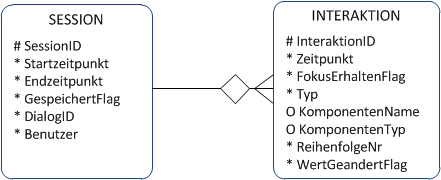
\includegraphics[scale=1]{img/ERM_UIDataCollector.png}
  \caption{Entity Relationship Model des UIDataCollectors nach Barker Notation \citep[vgl.][]{Inguanez2012}}
  \label{fig:ermUIDataCollector}
  \caption*{\textbf{Quelle:} eigene Darstellung}
\end{figure}


\subsection{Test und Einführung}